We have conducted extensive experiments to validate 
the effectiveness of our pipeline approach for NER tasks. 

\subsection{Data}
We validate our system using four datasets belonging to the general, biomedical and cybersecurity domains.
We use \data{OntoNotes5.0} and \data{WNUT17} for the general domain and \data{BioNLP13CG} for the biomedical domain, 
which are all publicly available.
For the cybersecurity domain, we use a private dataset, 
which contains news articles, blogs and technical reports related to malware, hacking groups and vulnerabilities.
We denote the dataset as \data{CyberThreats} in this paper.

We note that these datasets can demonstrate the effectiveness of our algorithms especially for non-word, low-resource (i.e., small number of training instances) entity types using the datasets from multiple domains and noisy text.
The datasets include not only traditional entity types with word mentions(e.g., PERSON, LOCATION) but also many entity types with non-word (Antivirus Signature) and very long mentions (e.g., URL, Software with version, etc).
Table \ref{tab:datasets_summary} shows a summary of the datasets.
\begin{table*}[h!]
\centering
\begin{small}
\begin{tabular}{ccccrrr}\toprule
 \textbf{Dataset} & \header{\#Entities} & \header{Non-Word} & \header{Low Resource} & \header{Train} & \header{Dev.} & \header{Test} \\ \toprule 
\data{BioNLP13CG} & 16 & Yes & Yes & 3,033  & 1,003 & 1,906 \\
\data{CyberThreats} & 8 & Yes & Yes & 38,721 & 6,322 & 9,837 \\
\data{OntoNotes5.0} & 18 & Yes & Yes & 115,812 & 15,680 & 12,217 \\  
\data{WNUT17} & 6 & Yes & Yes & 3,394 & 1,287 & 1,009\\
\bottomrule
\end{tabular}
\caption{Overview of the experimental datasets. \header{\#Entities} indicates the number of unique entity types.
\header{Non-Word} and \header{Low Resource} indicate if the dataset contains non-word mentions (e.g, mentions with digits and symbols) and low-resource entity types respectively.  
\header{Train}, \header{Dev.} and \header{Test} show the number of sentences in the datasets.}
\label{tab:datasets_summary}
\end{small}
\end{table*}

\yjcomment{Shall we show the class distribution for the datasets? We need to use the names of diffrent methods consistently. Let's make a name for our system instead of Span-Pipeline.}
\comment{Different domains (entity nature \& language context) / dataset sizes / No. of entities 
- BIONLP13CG: Bio dataset (using Scibert + BERT model)
- OntoNotes: General entities / newswire (using Roberta base)
- WNUT17: emerging entities from tweets (using BERT)
Also show from result analysis that span class is simpler and gives above 90\% result where as detector is the main bottleneck}

%%%%%%%%%%%%%%%%%%%%%%%%%%%%%%%%%%%%%%%%%%%%%%%%%

\subsection{Experimental Setup}
We use \deptool{transformers}\footnote{https://github.com/huggingface/transformers} library from \deptool{HuggingFace} and \deptool{pytorch} for implementation. 
For general English corpora like \data{OntoNotes5.0} and \data{WNUT17}
and the cybersecurity data, we use a pretrained BERT model (bert-base-uncased\footnote{https://huggingface.co/bert-base-uncased}). 
For the biomedical dataset (\data{BioNLP13CG}), we use SciBERT
(scibert\_scivocab\_uncased\footnote{https://github.com/allenai/scibert}), a language model for scientific text~\cite{beltagy-etal-2019-scibert}. 

Note that. in all our experiments, we only use the BERT-Base architecture, which has around 110 million trainable parameters. 
The training data is randomly shuffled and a batch size of $16$ is used with post-padding. We fixed random seed to $42$ for replication.
For BERT-based models, we set the maximum sequence length to $256$ for \data{BioNLP13CG}, \data{CyberThreats} , and \data{WNUT17} and to $512$ for \data{OntoNotes5.0}. 


We use the cross entropy loss during training unless otherwise specified. 
The development set evaluation takes place at steps of 0.5 training epochs. We train the models for $300$ epochs at learning rate $10^{-5}$ unless otherwise specified.
The BERT-based models output entity labels for each sub-token (as per WordPiece tokenization) of an existing token in the dataset. 
We take the label of the first sub-token as the label for the corresponding token for the evaluations.
We use Nvidia GeForce GTX 1080 and Nvidia Tesla V100 GPUs for model training and evaluation.

%%%%%%%%%%%%%%%%%%%%%%%%%%%%%%%%%%%%%%%%%%%%%%%%%

\subsection{Baseline Systems}
\yjcomment{Jatin -- please update this section}


We present this comparison since QA model serves as the primary backbone of our span-based approach. 
All models here use BIOE tagging scheme.
For span detection, we use \textit{Extract important entity spans from the following text} as the question irrespective of the entity types.
For span classification, we use \textit{What is $<mention>$} where $<mention>$ is the string value for an extracted span by the span detection model.  

\if false  
\texttt{BERT}: Proposed by \cite{devlin2018bert}, BERT is a bidirectional encoder transformer\cite{vaswani2017attention}. It applies WordPiece\cite{wu2016google} tokenization on input sentence which is then passed through several encoder layers with multiple attention heads capturing sentence semantics and inter-token relationships well. The model outputs contextualized embeddings for each sub-token in the sentence. We take the last hidden layer outputs from BERT model and pass it to a fully connected layer. The outputs are converted to a probability distribution over labels space. Model parameters are initialized from a pretrained model and fine-tuned on our NER task.


\texttt{BERT-Freeze}: To understand how much semantic information is already captured in a pretrained BERT model, we use the exact same architecture as \texttt{BERT} model above but freeze the BERT model parameters. So, the only trainable parameters remain from the fully connected layer. For this setting, we use learning rate as $0.005$.

\texttt{CNN-LSTM-CRF}: \comment{better to include this as a baseline since it is very widely used}
\fi

\subsection{Performance Comparison}
We compare the performances of our system, the baseline systems and the best reported 
state-of-the-art (SOTA) tools. 
All of our models' results were measured on the test sets using the model checkpoint corresponding to the best Micro F1-score on the development sets. 
Table~\ref{tab:res_span} shows the comparison results based on the mention-level Micro F1 scores on the test sets (i.e., only the exact matches are considered correct).
\begin{table*}[h!]
\centering
\begin{small}
\begin{tabular}{ccccc}\toprule
 \textbf{Model} & \texttt{BioNLP13CG} & \texttt{CyberThreats} & \texttt{OntoNotes} & \texttt{WNUT17} \\ \toprule 
BERT-QA & 86.69 & \textcolor{blue}{ongoing(y1)} & \textcolor{blue}{ongoing(j)}  & 44.60 \\
BERT-Span-Pipeline-Vanilla     & 86.69 & \textcolor{red}{todo} & 90.12 & 55.36  \\
BERT-Span-Pipeline     & 86.70 & \textcolor{red}{todo} & 90.31 & 56.30  \\
Reported SOTA & 85.56(thesis see) & N/A & 92.07(MRC-Dice) & 60.45(CL-KL)  \\
\bottomrule
\end{tabular}
\caption{Comparison of the NER results on the four datasets. The numbers indicate the mention-level Micro F1 scores. 
\yjcomment{can you find the results of SOTA without any external data or additional pretraining? I consider MRC-Dice also using additional info. as they added several synonyms/hyponyms in query.   we can put SOTA without external data and with external data in separate rows if you like. We point out that our system does not rely on external knowledge which is usually unavailable for domain-specific data and needs less computing resources than MRC}}
\label{tab:main}
\end{small}
\end{table*}

\paragraph{Feature Analysis}
To investigate the effectiveness of the character sequence and pattern embeddings,
we performed the span detection tasks with and without the character and pattern features.
In Table~\ref{tab:det_ablation}, we report the mention-level precision (P), recall (R) and F1 scores
by the two models. 
As we can from the results, adding pattern and character features improve the precision while
maintaining similar recall levels.
\begin{table*}[h!]
\centering
\begin{small}
\begin{tabular}{ccccccccccccc}\toprule
 \multirow{2}{*}{\textbf{Model}} & \multicolumn{3}{c}{\data{BioNLP13CG}} & \multicolumn{3}{c}{\data{CyberThreats}} & \multicolumn{3}{c}{\data{OntoNotes5.0}} & \multicolumn{3}{c}{\data{WNUT17}} \\ \cmidrule{2-12} 
 & P & R & F1 & P & R & F1 & P & R & F1 & P & R & F1 \\ \midrule
Char-Pattern & 91.43 & 90.70 & 91.06 & & & 78.63 \textcolor{blue}{ongoing(y4)}& & & 92.50 & & & 55.21  \\
No Char-Pattern& & & 90.67 &79.65 & 77.77 & 78.70 & & & 92.37 & 72.63 & 44.06 &54.85  \\
\bottomrule
\end{tabular}
\caption{Performance comparison of span detection with and without character and pattern embeddings}
\label{tab:det_ablation}
\end{small}
\end{table*}


\paragraph{Loss Function}
A recent study has shown that using dice coefficient as the loss function was more beneficial than 
the cross entropy loss for NLP tasks with imbalanced data~\cite{li2019dice}. 
Inspired by this work, we trained our span classification model, which has the data imbalance problem,
using both cross entropy loss and dice loss.
Our experiments also confirm that the dice loss provides a small improvement over the cross entropy loss 
as shown in Table~\ref{tab:class_ablation}.
\begin{table*}[h!]
\centering
\begin{small}
\begin{tabular}{ccccc}\toprule
 \textbf{Model} & \texttt{BioNLP13CG} & \texttt{CyberThreats} & \texttt{OntoNotes} & \texttt{WNUT17} \\ \toprule 
Span-Classification-Dice & 94.27 & 87.84 &  96.74 & 73.40  \\
Span-Class-CE     & 94.04 & 87.58 & 96.50 & 73.31  \\
\bottomrule
\end{tabular}
\caption{Span Classification Results with different loss functions}
\label{tab:class_ablation}
\end{small}
\end{table*}

\paragraph{Training Time}
As discussed in Section~\ref{sec:method}, our pipeline approach applying span detection  and span classification separately is more efficient than combined models.
To validate the assertion, we measured the training times of our pipeline system
and the baseline BERT-QA, which uses exactly the same features and underlying architecture but performs span detection and classification in one unified model.
All experiments were done using two V100 GPUs with 16G memory on each GPU. 
The results confirm that the pipeline approach is much more efficient,
and, the efficiency improvement grows as the size of training data and 
the number of entity types grow.
\begin{table*}[h!]
\centering
\begin{small}
\begin{tabular}{ccccc}\toprule
 \textbf{Model} & \texttt{BioNLP13CG} & \texttt{CyberThreats(10\%)} & \texttt{OntoNotes(10\%)} & \texttt{WNUT17} \\ \toprule 
BERT-QA                & 1,372.8 & 877.1 &  7,381.8   & 568.2\\
Span-Pipeline     & 241.2 (106.3/134.9) & 145.53 (113.7/31.9) & 300.8 (185.5/115.3)  & 122.9 (98.9/24.0)\\
\bottomrule
\end{tabular}
\caption{Comparison of the training time between our method and a non-pipeline QA-based NER method. 
    The training time is reported in seconds per training epoch. The numbers in the parentheses denote the training times for span detection and span classification respectively. }
\label{tab:train_time_ablation}
\end{small}
\end{table*}

\begin{table*}[h!]
\centering
\begin{small}
\begin{tabular}{cccccc}\toprule
      &  \textbf{} & BioNLP13CG & JNLPBA & CoNLL2003 & OntoNotes5.0\\\toprule
\multirow{3}{*}{Baseline} & \texttt{BERT-Freeze} &  75.42 & 55.93 & 82.79 & 67.35 \\
                          & \texttt{BERT} & 85.99 & 74.35 & 91.36 & 83.39 \\ 
                          & \texttt{BERT-QA} & \textbf{86.45} & 74.81 & 91.17 & \\\midrule
\multirow{3}{*}{OurModel} &        \texttt{Span Detection} & 90.12 & 78.35 & 95.23 & \\
        & \texttt{Span Classification} & 94.06 & 95.08 & 94.50 & \\
        & \texttt{Pipeline} & 85.89 & \textbf{75.01} & \textbf{91.64} & \\ \bottomrule
\end{tabular}
\caption{The classificaiton results of our system and the state of the art method over 4 benchmark datasets. 
     The numbers reprent the Micro-F1 in \% on the test datasets.}
    \label{tab:res_span}
\end{small}
\end{table*}

%\comment{need more results and some plots}

\if false
Next, we deep dive into the \texttt{BioNLP13CG} dataset which has $16$ entity types including several high and low-resource types. We compare the model performance at the entity type level for our 3 major NER approaches: sequence labeling, question answering and span-based pipeline. We compare our best performing model variants through entity-level and macro-averaged F1-scores. Let $\mathcal{T}$ be the set of all entity types and F1$_t$ be the F1-score for individual entity type $t \in \mathcal{T}$. Then, Macro-averaged F1-Score is defined in Equation \ref{eq:macro_f1} as:
\begin{equation}
\label{eq:macro_f1}
    \text{Macro-F1} = \frac{1}{\mathcal{\vert\mathcal{T}\vert}}\,\sum_{t\,\in\,\mathcal{T}}{\text{F1}_t}
\end{equation}
We present the comparison among the following models:
\begin{itemize}
    \item \texttt{Dice Loss}: Sequence labeling NER approach over BERT model with \texttt{BIO} tagging scheme and dice loss instead of cross entropy.

    \item \texttt{Special Symbol}: Sequence labeling NER approach over BERT with \texttt{BIO} tagging scheme and additional one-hot input feature to capture if a token is a special symbol like \textit{hyphen}, or \textit{parenthesis}.

    \item \texttt{BERT-QA (Where)}: Question answering NER approach with \texttt{BIOE} tagging scheme and \textit{Where} as the question word.

    \item \texttt{Span Based}: Pipelined approach which uses the QA setup with \texttt{BIOE} tagging scheme and \textit{What} as question word for span detection and QA-based sequence classification for span classification.
\end{itemize}

\begin{figure}
    \centering
    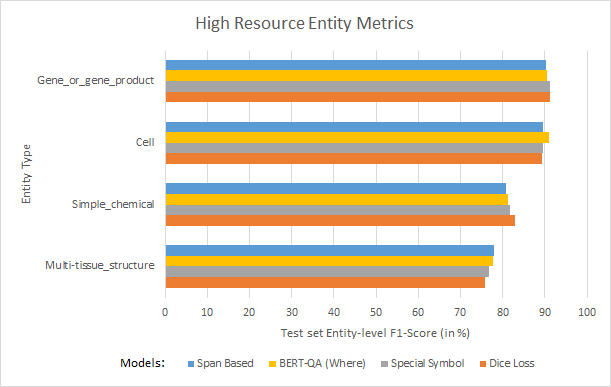
\includegraphics[scale=0.5]{../thesis/high_resource_entity_metrics}
    \caption{Test set Entity-level F1 scores for high resource entities in \texttt{BioNLP13CG} dataset}
    \label{fig:high_resource_entity_metrics}
\end{figure}

\begin{figure}
    \centering
    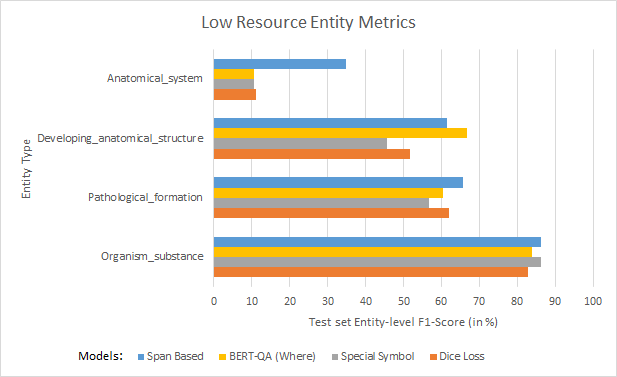
\includegraphics[scale=0.5]{../thesis/low_resource_entity_metrics}
    \caption{Test set Entity-level F1 scores for low resource entities in \texttt{BioNLP13CG} dataset}
    \label{fig:low_resource_entity_metrics}
\end{figure}

\fi
